%Git-rapport
\documentclass[a4paper]{article}

\usepackage[swedish]{babel}
\usepackage[utf8]{inputenc}
\usepackage{graphicx}
\setcounter{secnumdepth}{4}
\usepackage{titlesec}
\usepackage{caption}
\usepackage{float}
%For figures
\graphicspath{ {Figures/} }
\captionsetup{justification=centering}


\begin{document}
\begin{titlepage}
\centering
{\bfseries\huge Projektrapport DAT290}

\vspace{10mm}

{\Large Radiostyrd Bil, Grupp 07}

\vspace{20mm}

{\Large \itshape{Joakim Junttila, Johanna Gudmandsen, Gustav Holst,\\Henrik Klein Moberg, Anders Berggren Sjöblom, \\[1mm] Stanislaw Zwierzchowski, Carl Lundgren}}

\vspace{10mm}

%Vet ej vilket datum som ska stå
{DATUM}


\normalsize{
\begin{table}[b]
\centering
\begin{tabular}{|l|l|l|}  \hline
         & \bf Namn & \bf Datum   \\ \hline \hline
Granskad & NAMN     & DATUM        \\ \hline
Godkänd  & NAMN     & DATUM         \\ \hline
 \end{tabular} 
 \end{table}}
\end{titlepage}

\tableofcontents

\newpage
\section{Ordlista}
PWM-signaler(KÄLLA) - PWM eller Pulse Width Modulation är en moduleringsteknik och används mest för att styra mängden elektrisk ström som förs till, exempelvis, en motor.
%NÖDVÄNDIGT???? I varje period i en PWM-signal kan spänningen antingen vara 0, låg, eller 1, hög, och det som mottagaren svarar på är hur stor del av perioden som signalen var på högspänning. I detta projekt är maxspänningen ca 3, 4V, och motorerna svarar på en medelspänning mellan 250-450mV. Dessa medelvärden, eller dutycycles, styrs i bildatorn med hjälp av en av datorns timers och standardbibliotek för dessa

STMicroelectronics

Android Studio
MRX-242
MD407
ADC
Avståndsmätare
Potentiometer


\newpage
\section{Introduktion}

Radiostyrda bilar började produceras på mitten av 60-talet~\cite{RCHistory}. Under åren har de både tävlats med samt varit en väletablerad leksak till barn. Trots att den genomgått mindre justeringar har den radiostyrda bilens uppbyggnad i det stora hela förblivit densamma.

\subsection{Syfte}

Syftet med detta projekt är att uppdatera den klassiska radiostyrda bilen genom att ersätta befintlig sändare samt mottagare i en radiostyrd bil med nya datorer samt även möjliggöra styrning från en Andriodtelefon. Intentionen är även att implementera en kontrollapplikation som ska kunna stoppa bilen från att kollidera.


%Syftet med detta projekt är att uppdatera den klassiska radiostyrda bilen med hjälp av ny teknik som bluetooth. För att följaktligen erhålla en mer modern teknisk produkt.

\subsection{Mål}
Målen nedan beskriver konkret vad som ska uppnås med projektet.

\begin{itemize}
\item Den befintliga sändaren samt mottagaren som finns i handkontrollen respektive bilens elektronik ska bytas ut mot ARM-baserade system(se Figur 1). Dessa ska vid färdig produkt kontrolleras via Bluetooth.
\item En kontrollapplikation ska implementeras. Med hjälp av enn avståndsmätare(se Figur 1) är avsikten att bilen självständigt ska kunna köra rakt fram i högsta möjliga hastighet och på ett avstånd av maximalt 1 cm från en vägg bromsa in helt utan att kollidera. Kontrollapplikationen styrs via Bluetooth.
\item Styrning via mobilapplikation implementeras. Bilen ska då kunna manövreras genom ett Andriodsystem via Bluetooth.
\end{itemize}

\begin{figure}[H]
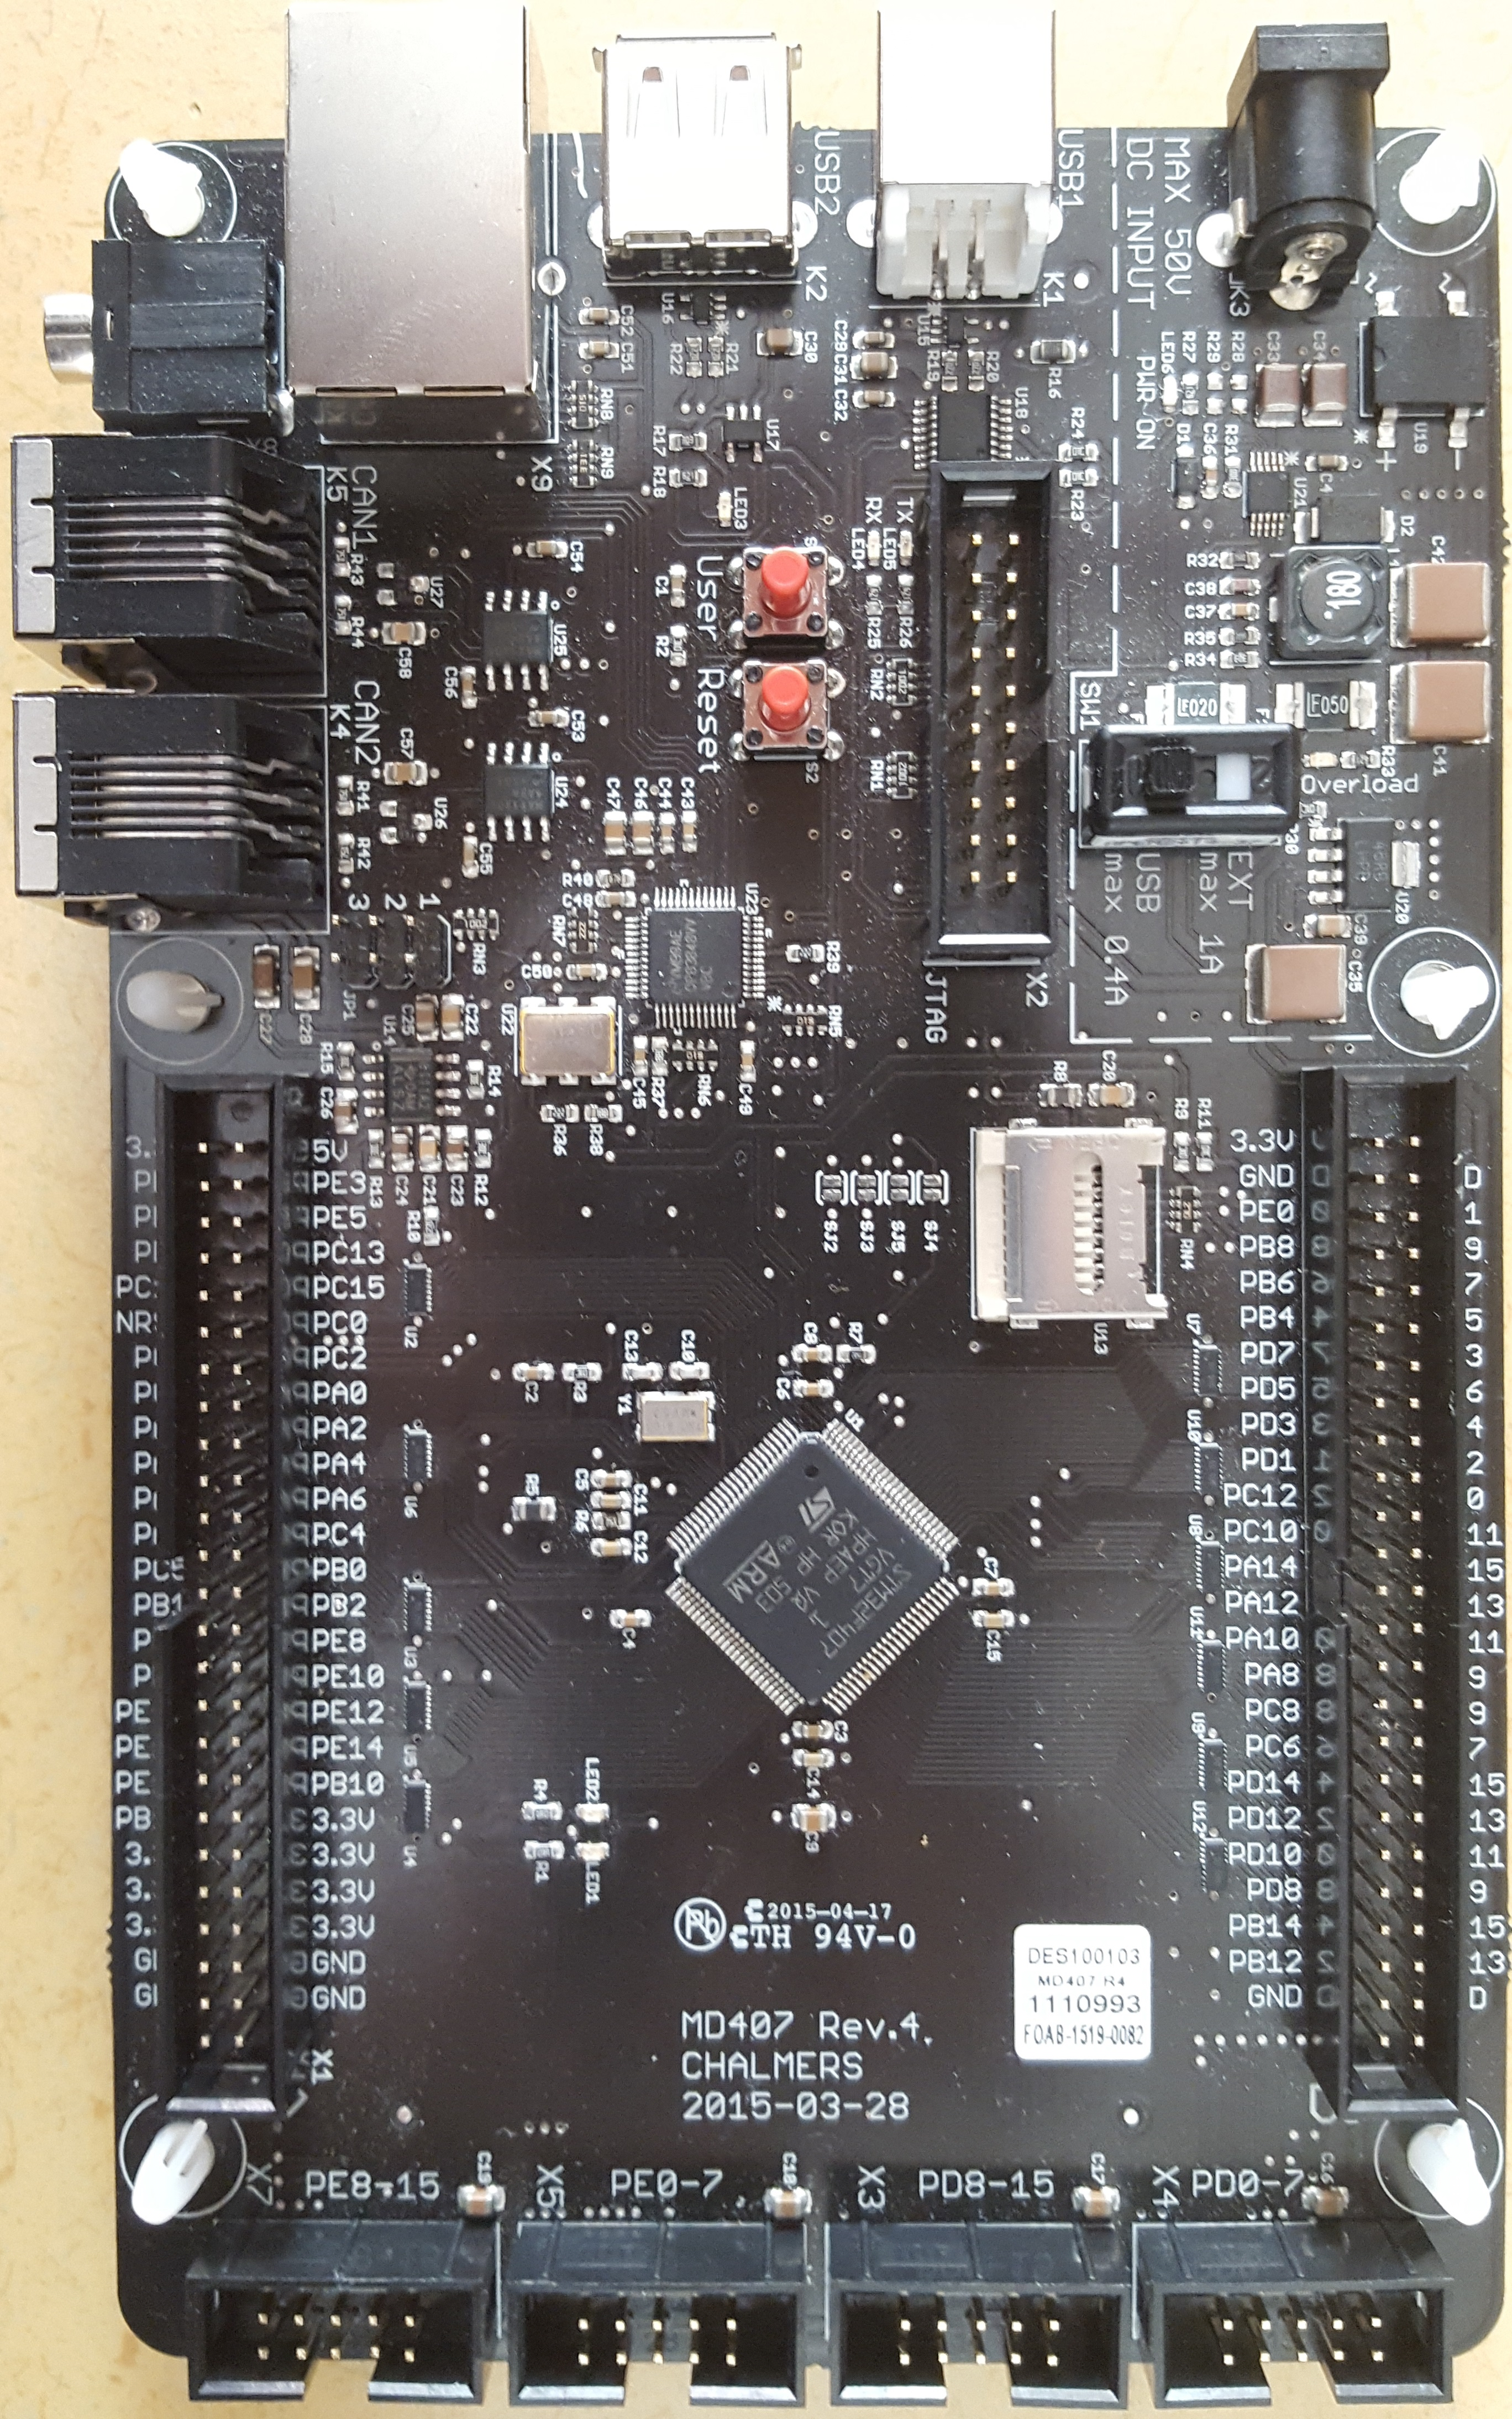
\includegraphics[scale=0.04]{MD407.jpg}
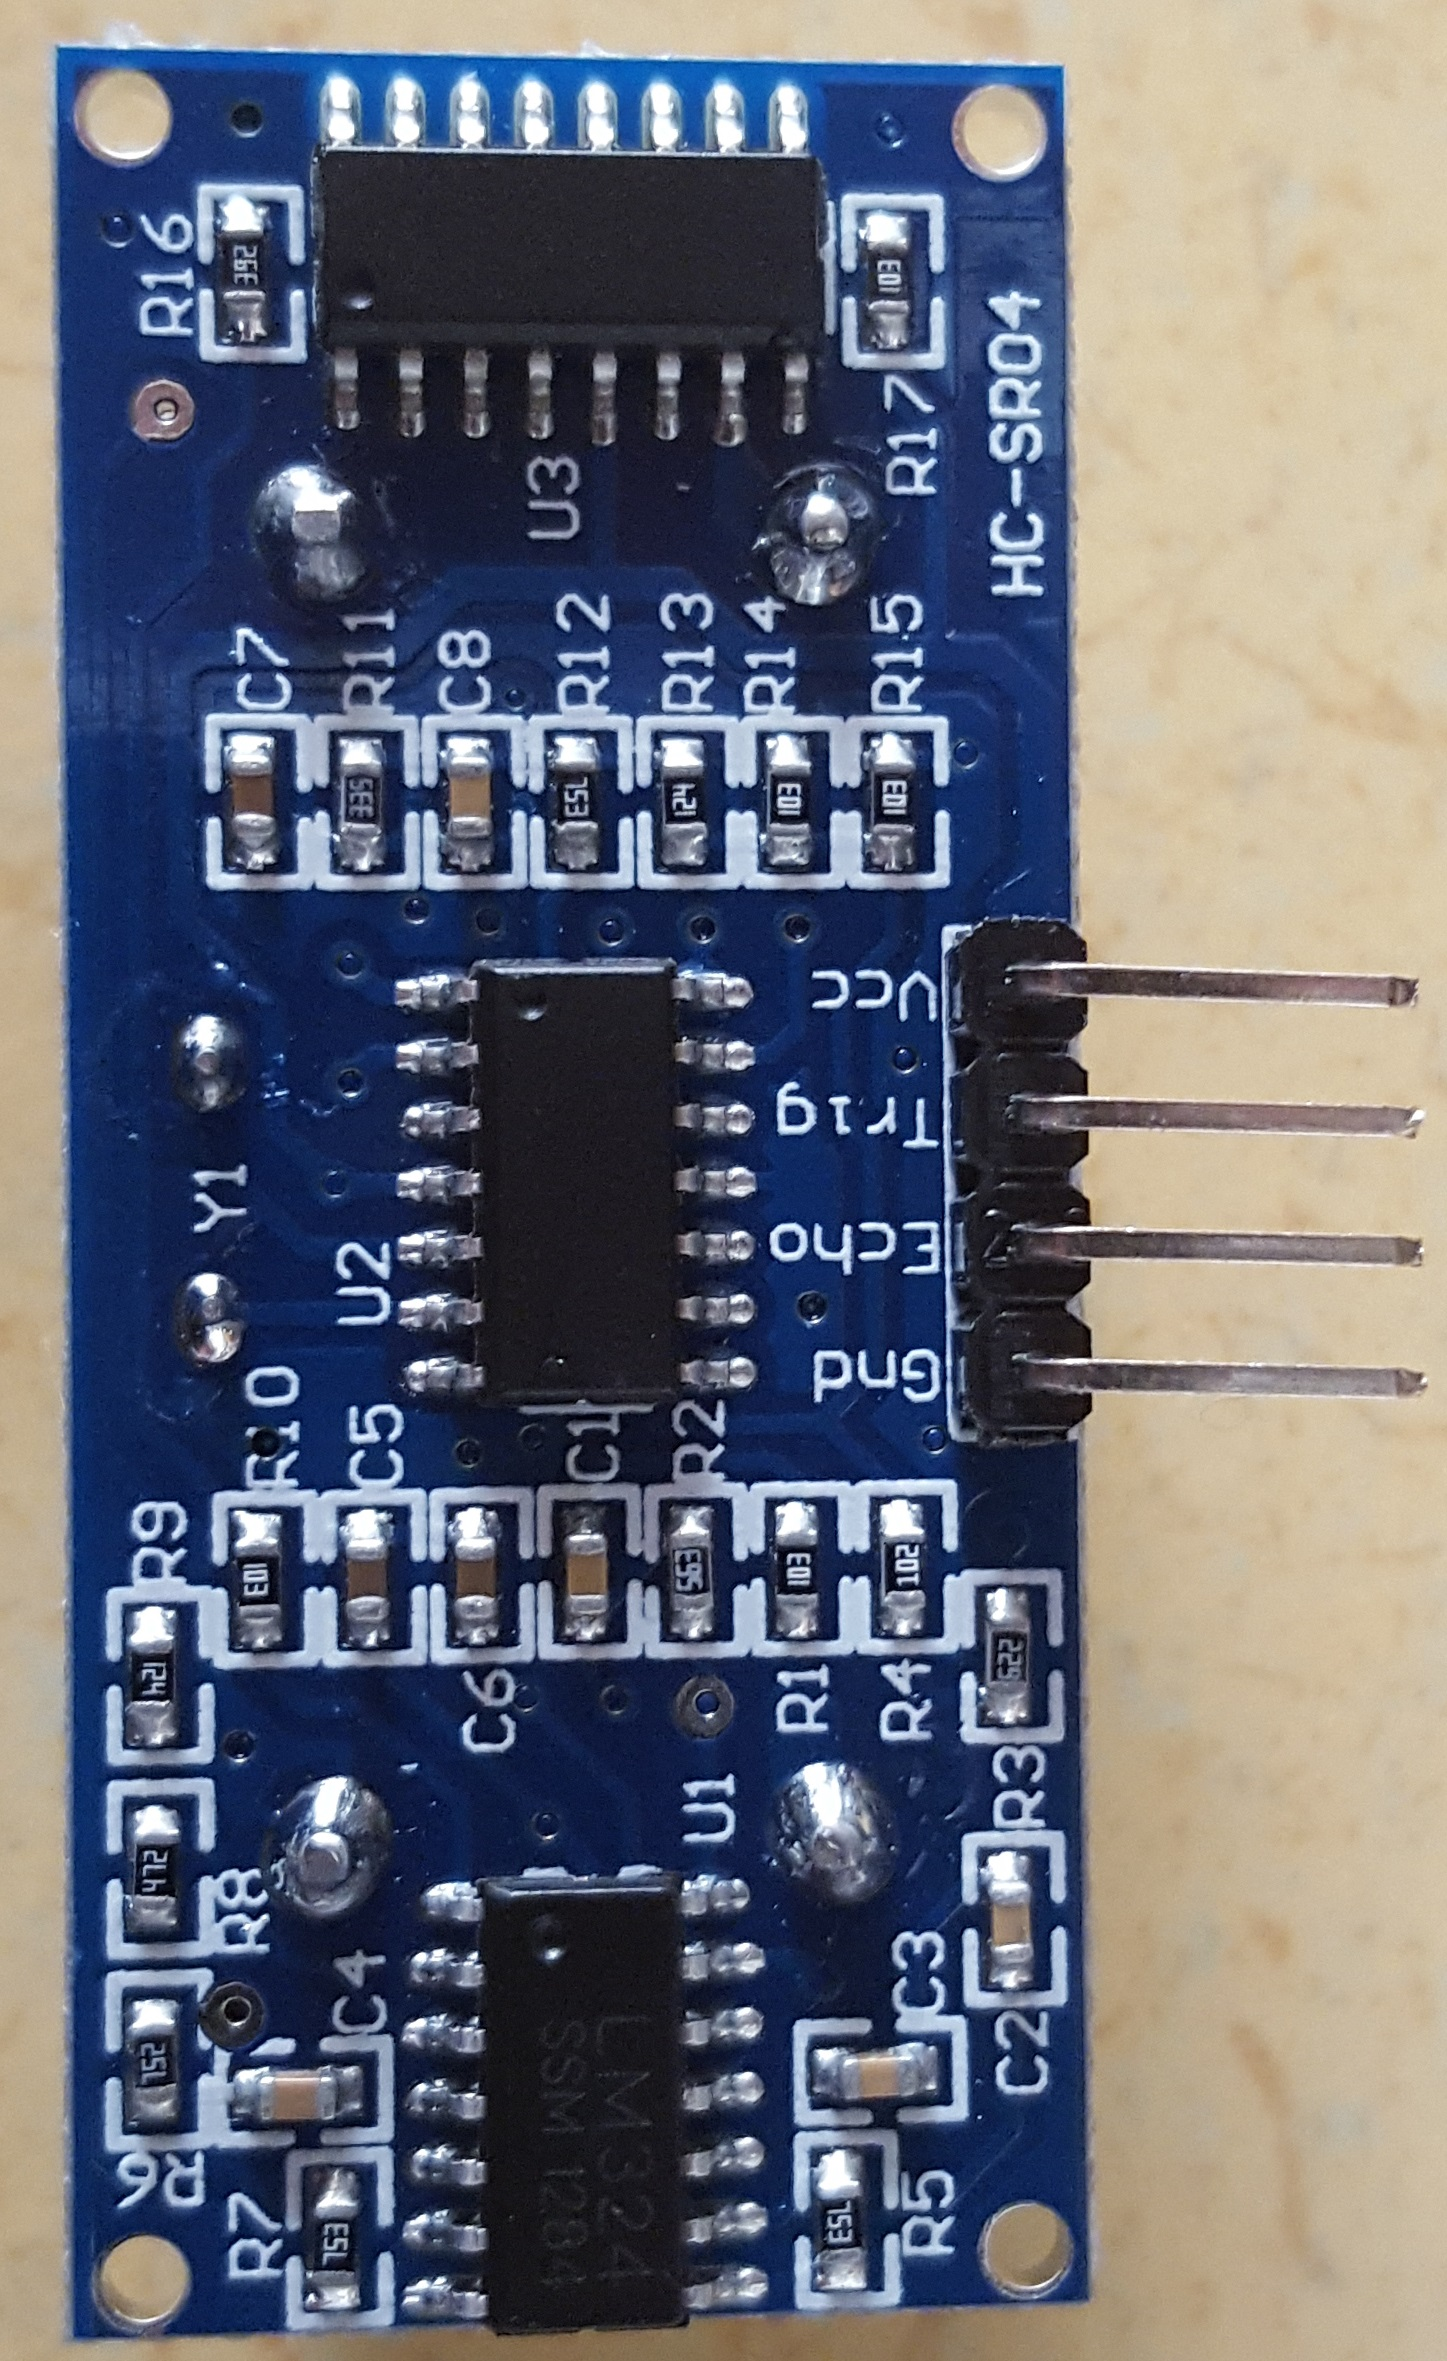
\includegraphics[scale=0.07]{DistanceMeasure.jpg}
\centering
\caption{\it MD407, en ARM-dator(vänster), Avståndsmätare(höger).}
\end{figure} 

%Målförslag
%Projektet går ut på att ersätta delar av elektroniken i en radiostyrd bil. Sändaren samt mottagaren som finns i handkontrollen ska bytas ut till en ny handkontroll. Nya handkontrollens sändnings singnal kommer ändras till att slutligen bli  Bluetooth. I samband med singnal bytet kommer nya handkontrollen att anpassad till andara ändringar som ska genomföras. Andra ändringar som ker berör bland annat skälva bilen. Bilens elektronik ska bytas ut mot ARM-baserade system. Vidare ska en kontrollapplikation implementeras i bilen med hjälp av ett antal avståndsmätare. Därefter ska bilen programeras så den självständigt ska kunna köra rakt fram i högsta möjliga takt och bromsa in helt på ett avstånd av maximalt 1 cm från en vägg. Sista steget i arbetsprosessen är att med hjälp av Bluetooth signalen utveckla en aplickation som ska kunna styra bilen och fungera som en fullfjädrad handkontroll.

\subsection{Arbetsmetod}
\subsubsection{Uppmätning av styrsignaler}
%Förklara hur de genererats
Projektet inleddes med att mäta upp befintliga styrsignaler. För att kunna replikera signalerna som ursprungligen skickas från mottagare till bilens styrelektronik kopplas ett kretskort(VILKET) till bilens egna kontrollenhet, MRX242. Kretskortet har möjlighet att dela på mottagarens signaler och kopplat till ett oscilloskop kan specifika signaler tydligt mätas upp. Signalerna är av typen PWM och uppmäts i Volt. 


\subsubsection{Konfiguration av ny sändare}
\vspace{5mm} \noindent
Datorenheten MD407 ersätter sändaren. Enheten kopplas till en potentiometer genom en bred sladd från datorenheten till potentiometerns tio vänstra pinnar(se Figur 2). På potentiometerns mellersta pinnar finns tre kolumner. Ström till de vridbara kontakterna erhålls genom enligt Figur 2 koppla korta sladdar mellan kolumn 2 och de övriga kolumnerna. Följt av detta kopplas en sladd från en pinne på den övriga kolumnen i samma rad som den korta sladden till PC1-porten och PC2-porten på MD407. De styr motorn och servot i den angivna ordningen. Koden till detta har är skriven i C med utvecklingsmiljön Codelite.



\begin{figure}[H]
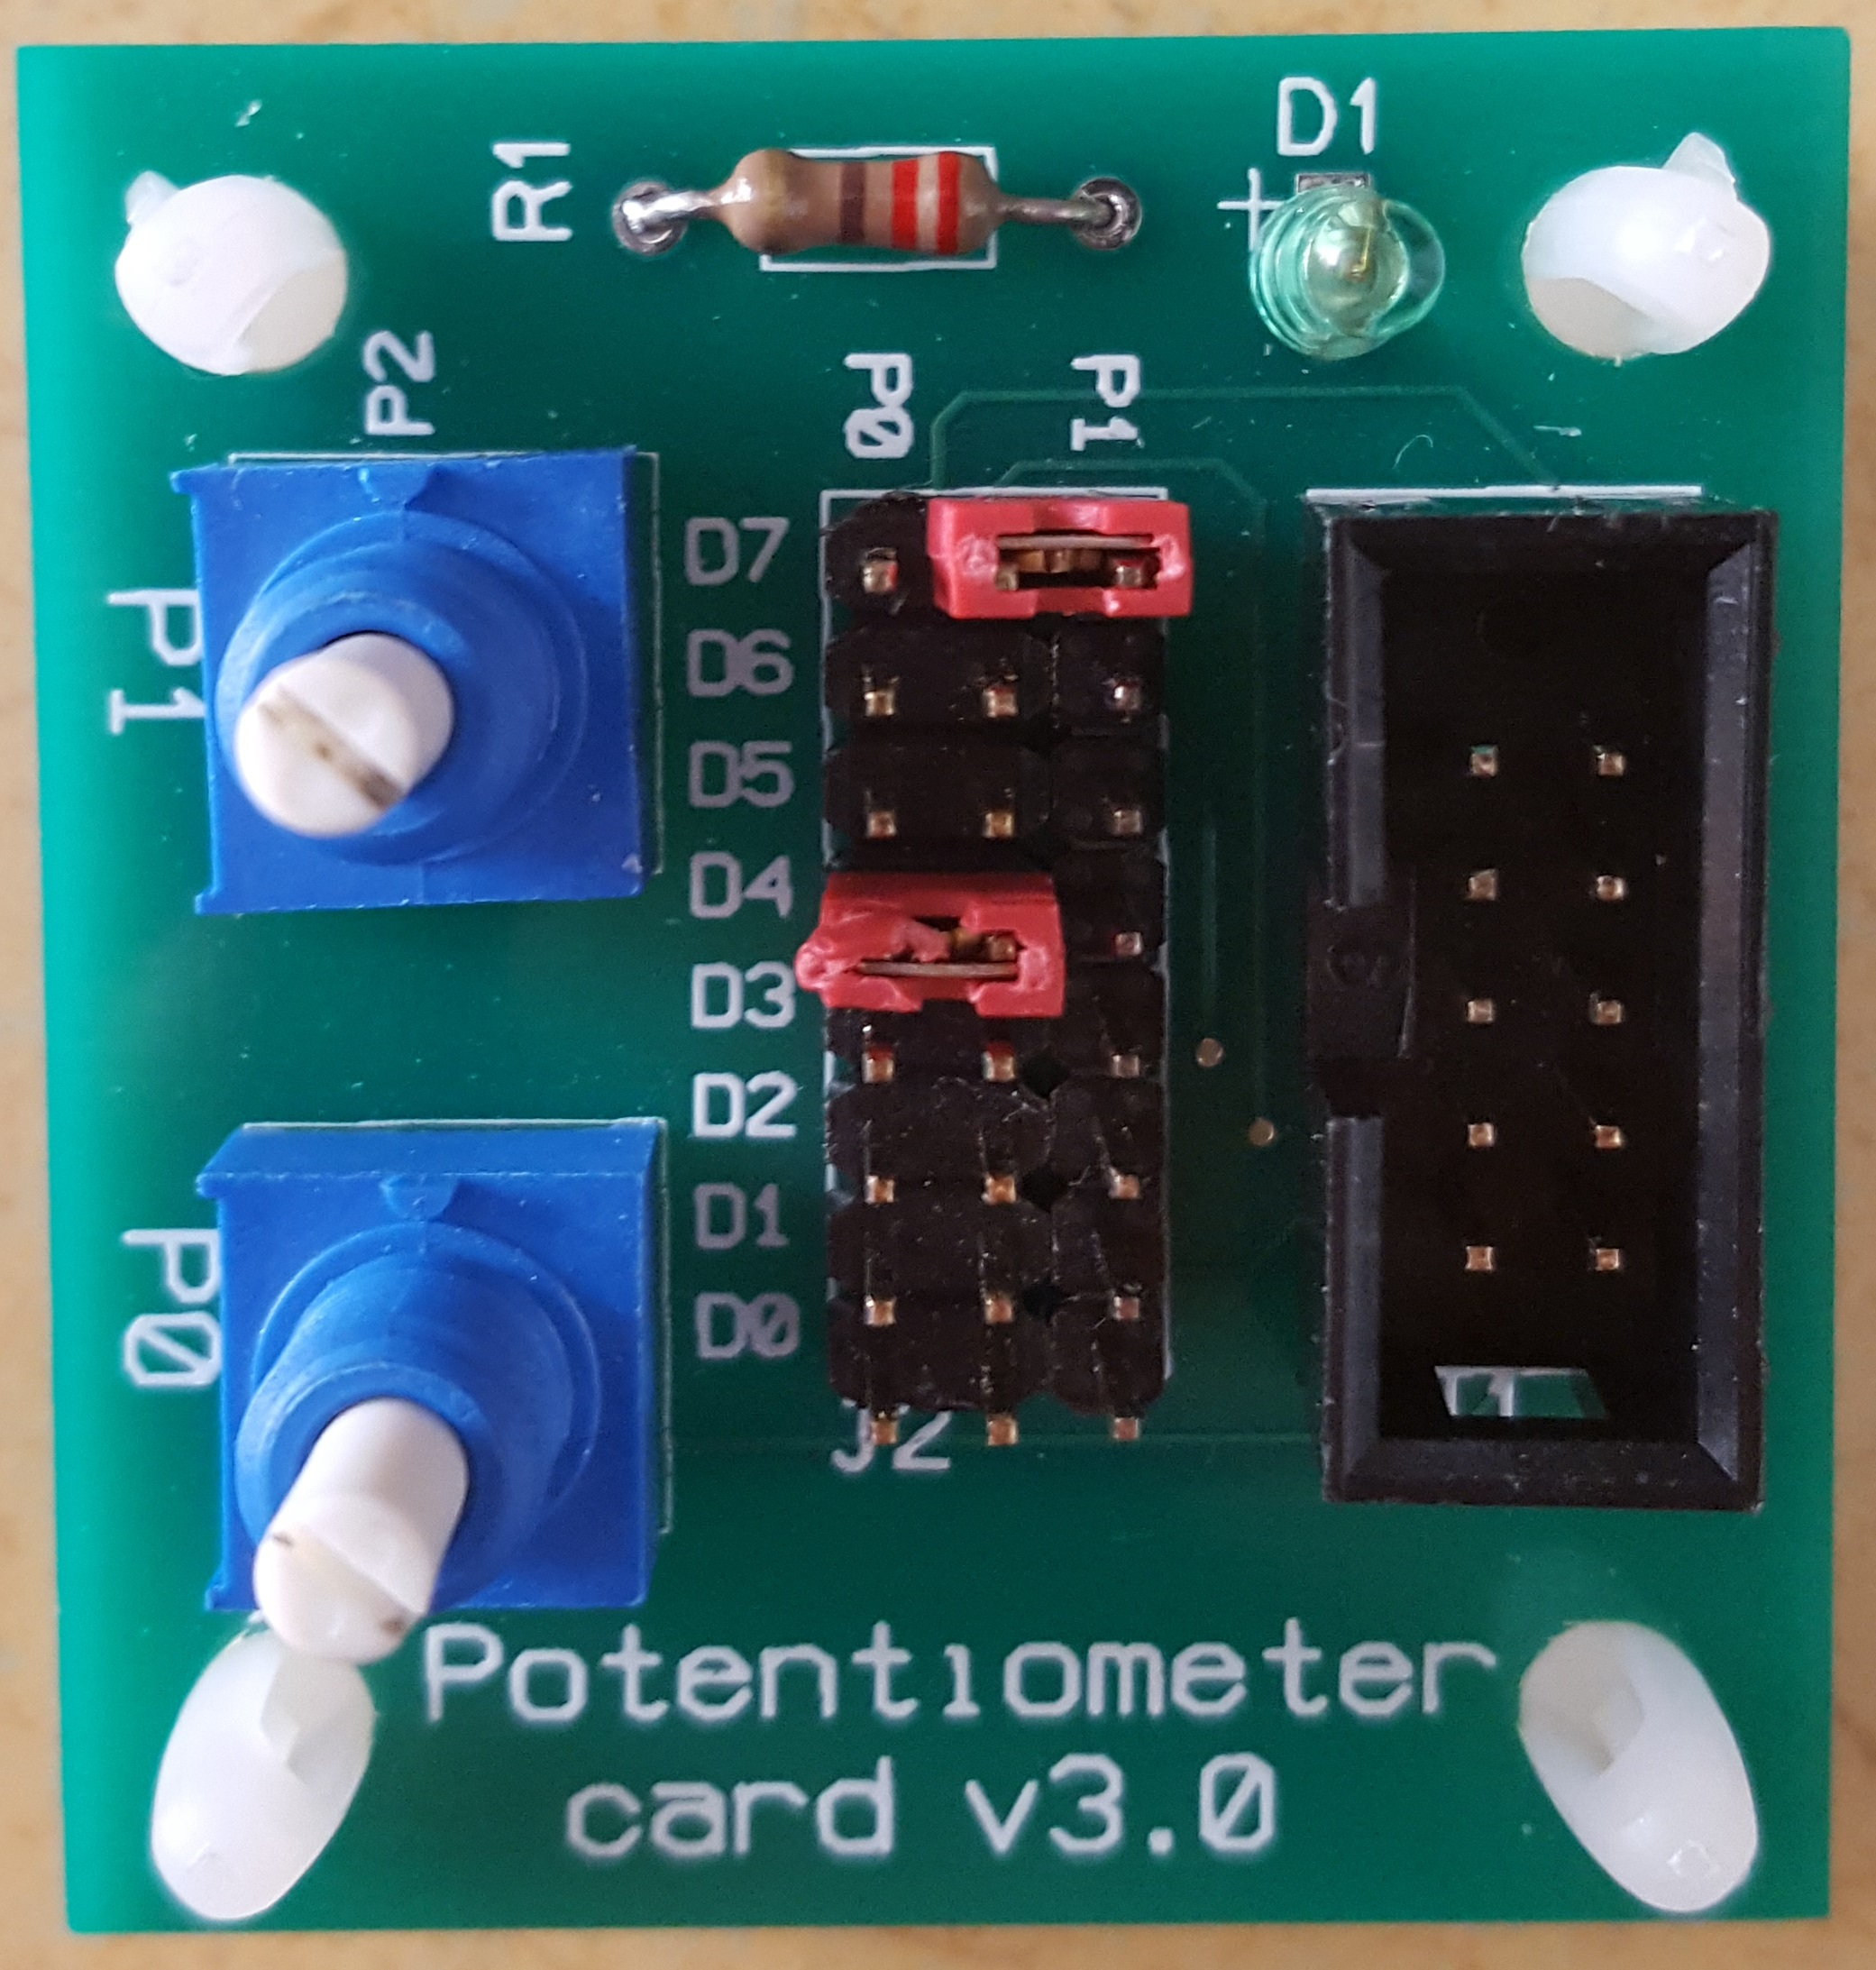
\includegraphics[scale=0.05]{Potentiometer.jpg}
\centering
\caption{\it Potentiometer.}
\end{figure} 

\subsubsection{Hur sändare och mottagare kopplas samman}
\vspace{5mm} \noindent
Båda datorenheterna kopplas sedan samman. Med hjälp av programmet ETERM kan USART genom USB koppla två bärbara datorer till sändare och mottagare för att aktivt kunna använda C-koden till att utföra operationer. PA0-porten på sändaren kopplas till kretskortet UART4 som i sin tur kopplas till en radiofrekvenssändare, en identisk procedur görs på mottagaren men på PB11-porten med kretskortet UART4 och en radiofrekvensmottagare. Radioenheterna benämns som RF-mottagare och RF-sändare. Stöd från hjälpfunktioner i biblioteket(NAMN) möjliggör för att kunna skriva till PA0-porten och läsa från PB11-porten. Koden är även här utvecklad i Codelite.

%TILL DELSYSTEM


\subsubsection{Konfiguration av ny mottagare}
\vspace{5mm} \noindent
En ytterligare datorenhet, MD407, ersätter mottagaren i bilen. Portarna CH3 och CH4 på kretskortet TIM2 kopplas till PA2 respektive PA3(se Figur 1) på den nya mottagaren. Koden, skriven i C med utvecklingsmiljön Codelite, initierar CH3 till att reglera motorstyrningen och CH4 till att kontrollera rattutslagen. När RF-mottagaren tar emot ett meddelande startas en funktion. Denna funktion undersöker vilket kommando som ska utföras samt till vilken grad detta skall göras. Exempelvis, erhåller mottagaren kommandot att bilen ska ändra motorhastigheten beror hastigheten på storleken av värdet. Mottagaren är kopplad direkt till bilens styrelektronik, en sladd till motorn och en till styrservot. När värdet på meddelandet från sändaren erhållits skickas en PWM-signal till den önskade styrelektroniken i bilen som fångar upp dessa under en period, uppfattar värdet och agerar.

%TILL RESULTAT
%För att informationsutbytet ska fungera utan att störningar kommer emellan meddelandena skickas signaler ungefär 100 gånger per sekund och de tas emot med samma hastighet


%Kretskortet konfigureras till att mäta signalerna från den ursprungliga kontrollenheten i bilen med hjälp av ett oscilloskop.



%Förklara mer ingående. Mycket mer ingående
%\vspace{5mm} \noindent
%Resultatet av detta användes i utvecklandet av ett program som själv kunnat generera samma slags signaler genom en ARM-processor kopplad till bilen. Programmet är skrivet i C i utvecklingsmiljön CodeLite.

%Lägg till referens på "motorernas respons på signalerna är..." samt "STMicroelectronics" BYTA TILL SYSTEMÖVERSIKT, LITE AV DENNA
%\vspace{5mm} \noindent
%Signalerna som ska avläsas och sedan genereras är av typen PWM (Pulse Width Modulation. Med detta menas att det som ska avläsas på oscilloskopet är hur mycket av signalen som är på maxspänning jämfört med en hel period av radiovågorna. Det som möjliggör avläsningen av signalerna samtidigt som det går att se motorernas respons på signalerna är ett kretskort som delar på signalerna. Efter avläsningen replikeras dessa signaler i vår datorenhet, MD407, för att sedan kunna skickas från datorn direkt till mottagaren i bilen varpå bilen ska ge samma respons som med den ursprungliga sändaren. Detta arbete har förenklats med hjälp av kodbibliotek från STMicroelectronics som innehåller funktioner för att initiera PWM-genererande.

\subsubsection{Komplettering med applikation som sändare}
\vspace{5mm} \noindent
Mobilapplikationen ska vara funktionell på en Andriodtelefon och kopplas till den radiostyrda bilen via Bluetooth. Arbetet inleddes genom att studera bilens ultraljudssensor varpå en planering för sensorns användning har skrivits(?????). Två applikationer konstruerades separat; en GUI med olika reglage för att styra hastighet och riktning, samt en applikation som kontrollerar Bluetooth. Dessa skrevs i Java genom Eclipse och importerades till Android Studio.

\newpage
\section{Teknisk beskrivning}

\subsection{Teknisk bakgrund}
För att kunna kontrollera en radiobil används en sändare och en mottagare~\cite{RCTechnique}. Radiosignaler på en okänd frekvens skickas från sändaren och avkodas av mottagaren i radiobilen. Dessa omvandlas då till elektroniska signaler som antingen kontrollerar bilens hastighet eller riktning. Parallellt med detta styrs även bilens hastighet av motorns kraftutslag, medan riktningen beror på hjulens gradförskjutning. Genom en ytterligare signal kan bilens hastighet även reverseras. Bilens styrenhet omvandlar radiosignaler som sedan kontrollerar bilens rörelse.

\subsubsection{Nya styrsignaler}
Bilens styrsignaler kontrolleras av en kontrollenhet~\cite{projektDir}. Enheten fungerar simultant som radiomottagare och styrsignalgenerator. Utöver detta generar den signaler till båda motorerna i bilen via tre kablar. I mening att ersätta dessa med nya signaler finns även tillgång till ett ytterligare kopplingsblock.


\subsection{Systemöversikt}
Systemet har två huvuddelar, en MD407-enhet samt en Androidapplikationen som båda  kan agera handkontroll och bildatorn som genererar signaler till motorerna.


\subsection{Delsystem}
\subsubsection{Specifikation av nya styrsignaler}
Styrsignalerna uppmättes med hjälp av oscilloskop. Cykelmedelvärdet för mV vid styrning när rattutslaget är maximalt åt vänster respektive höger gick från 250mV till 450mV. Samma värde på hastigheten angav att full hastighet bakåt är av storleken 265mV, bilen är i neutralt läge vid 410mV och de maximala hastigheten nås vid 530mV. Genom att dividera dessa värden enskilt med den maximala volten(3.4V) som kan skickas från pinnarna på datorenheten, MD407, och multiplicera med perioden erhålls det värde bilens styrelektronik läser av. Detta resulterar i att bilen lyssnar på värden mellan 110-173(ENHET) under perioden av 1388(ENHET).

\subsubsection{Specifikation av PWM-signaler}
PWM-signalerna är specificerade att upptäckas på specifika värden. I varje period i en PWM-signal kan spänningen antingen vara 0, låg, eller 1, hög, och det som mottagaren svarar på är hur stor del av perioden som signalen var på högspänning. Maxspänningen pinnarna i MD407 skickar är ungefär 3.4V och elektroniken i bilen svarar på en medelspänning mellan 250-450mV. Dessa medelvärden, eller dutycycles, styrs i bildatorn med hjälp av en av datorns timers och standardbibliotek för dessa

\subsubsection{Sändare: Androidapplikation}
Androidapplikationen agerar som en handkontroll. Av denna krävs att skicka bytes seriellt till bilens dator med en Bluetooth-länk för att därmed erhålla den sökta trådlösheten(källa??? behövs det???). Detta följer protokoll som bestämts av projektspecifikationer(SOM STÅR VAR?) där de två mest signifikanta bitarna i varje byte bestämmer vilken sorts signal som ska ändras, till exempel styrning, drivmotor eller initiera kontrollapplikationen. Mobilapplikationen har på skärmen virtuella reglage som ska emulera ordinarie handkontrollens analoga funktion så att exempelvis hastighetsövergången är så jämn som möjligt.

\subsubsection{Sändare: MD407-enhet via RF}
Datorenheten MD407 kopplas till potentiometer för att ge den ström. De trekolumnerna av pinnar som finns i mitten på potentiometern(se Figur 2) använts till olika ändamål. Den mittersta kolumnen möjliggör för ström, därav får de vridbara kontakterna på potentiometern ström genom de korta sladdarna mellan strömkolumen till respektive vridkontakt. Sladden från den sista kolumnen på samma rad kopplat till MD407 ger värden konstant till datorenheten. På denna enhet finns en integrerad ADC. Denna tar emot värdena från portarna PC1 samt PC2 och översätter det till digitala värden. Genom RF-enheter kan de nya datorenheterna kommunicera. Resultatet skickas från sändarens RF-enhet en byte åt gången 100 gånger i sekunden till mottagarens RF-enhet. Specifikationerna som följs är att de första 2 bitarna indikerar kommandot och de resterande 6 bitarna med vilket värde kommandot ska utföras. 

\subsubsection{Mottagare: MD407-enhet}
Signalerna som skickas från sändaren tas emot av en RF-mottagare((((generisk Bluetooth-modul))) som är kopplad till USART1-porten på mottagaren i bilen, en MD407-enhet. När programmet på denna dator startas måste datorn initialt skicka PWM-signaler som motsvarar neutralt läge för drivmotorn i en kort stund innan övriga signaler kan sändas. Efter detta kan mottagaren ta emot bytes från sändaren samt skicka PWM-signaler till bilens styrelektronik. De 2 mest signifakanta bitarna av byten mottagaren erhålligt har syftar på vilket kommando ska utföras. Detta värdet analyseras då i mening att skicka en PWM-signal till korrekt del i bilens styrelektronik. Värdet 1 eller 2 leder till att PWM-signalen skickas via en sladd från MD407 till bilens motor respektive styrservo. De 6 minst signifikanta bitarna har ett värde mellan 0-63 när mottagaren får de. Till detta adderas en offset av 110 vilket gör att värdet istället kommer befinna sig i intervallet 110-173. Detta värde skickas via sladden till den berörda styrelektroniken och uppfattas av bilen som svarar med korrekt funktionalitet. Syftar kommandot på motorn kommer bilen åka i högsta möjliga takt bakåt vid värdet 110. Farten minskar sen vid högre värden och bilen når neutralt värde vid 142. Värden över detta upp till 173 får bilen att öka i acceleration. Värden utanför detta intervall uppfattas inte av bilens elektronik. Värden till motorn inom intervallet omvandlas och får en medelspänning mellan 256-530mV som den direkt svarar på. En identisk procedur sker för värden till styrning där de som ligger i intervallet omvandlas och får en medelspänning mellan 250-450mV(RÄTTA EXAKTA VÄRDEN). Omvandlingen sker genom att dividera värdet från mottagaren med periodens längd, 1388, och multiplcera med maxspänningen, 3.4. Utöver detta kan en kontrollapplikation påbörjas(FORTSÄTT VID MER INFO). 


%Datorn i bilen tar då emot ett kommandokod från Bluetooth-länken och analyserar detta i mening att specificera vilket kommando de två bitarna syftar på ska utföras. PWM-signalerna ändras sedan efter värdet på kommandot, de sex minst signifikanta bitarna, eller påbörjar kontrollapplikationen för demonstration. Motorerna tar emot PWM-signalerna och ger utslag beroende på deras medelspänning.






\newpage
\section{Resultat}






\newpage
\section{Slutsats}



\newpage
%To references
\bibliographystyle{IEEEtran}
\bibliography{referenserRapport}


\end{document}

